\documentclass[12pt]{article}
\author{Mengxiao}
	\title{Cpts570-hw1}
	\usepackage{graphicx}
\begin{document}
	\maketitle
	\pagebreak
	\section{Analytical Part}
		\subsection{Problem 1}
			\par a. The decision boundary of voted perceptron is non-linear. The decision boundary would change with the change of the maximal value of the weight vectors.
			\par b. The decision boundary of average perceptron is linear.	We only need to compute the average of the weight, the average would be linear.
		\subsection{Problem 2}
			\par According to the class slides, the problem:
$$ w_{t+1} = \min\limits_w\frac{1}{2} ||w-w_t||^2$$
$$ s.t. y_t(w\cdot x_t)\geq M$$
			\par The Lagrangian:
$$ L(w,\tau)=\frac{1}{2} ||w-w_t||^2+\tau(M-y_t(w\cdot x_t)) $$
			\par Solve for the dual:	$\max\limits_{\tau\ge0}\min\limits_w\ L(w,\tau)$
			\par To the Dual Problem:
$$ \max\limits_{\tau\ge0}\ -\frac{1}{2}||x_t||^2\tau^2+\tau(M-y_t(w_t\cdot x_t))$$
			\par Finally, solve it:
$$ \tau = max\{0, \frac{1-y_t(w_t\cdot x_t)}{||x_t||^2}\} $$
		\subsection{Problem 3}
				\par\qquad a. I will put the weight $h_i$ as a part of $\tau$ that make the update formula like this: $w=w+(\tau\cdot h_i)\cdot(y_t\cdot x_t)$, so that everytime the weight $w$ needs update would consider the importance weight.
				\par b. Maybe I can repeat training the examples with higher importance weight, like If it's weight is $2$, I will train it twice. We can also let the importance weight times the input example if these examples are numerical.
		\subsection{Problem 4}
				\par\qquad a. We can cut down the $\tau$ when facing with the negative examples like let $\tau' = 0.1\tau or 0.05\tau$.
				\par b. I would try to use these positive multiple-times or do some translation to let the negative examples can be used for positive examples like take the negative of these negative examples.
 	\section{Programming and Empirical Analysis Part}
		\subsection {Binary Classification}
			\par a.	\par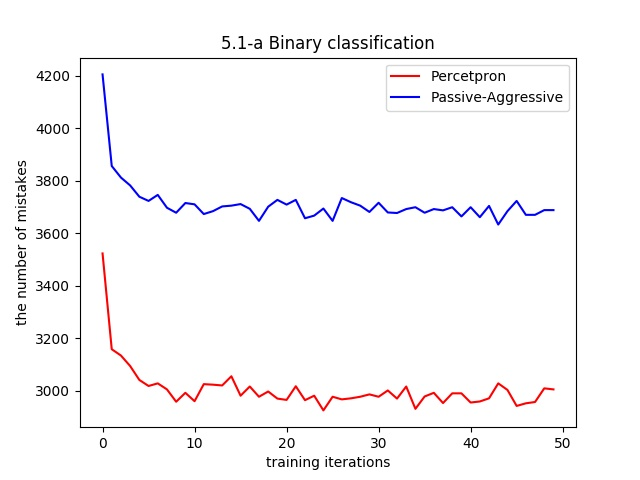
\includegraphics[height=10cm] {part1_a}
			\par I find that the number of mistake for Perceptron is less than Passive-Aggressive algorithm. The curve for Perceptron is shocking around 3,000  and the curve for PA is shocking around maybe 3,700, I think it is the limitation of their algorithm. 
			\par Also, the decline of mistakes is really quick, only need 5 iterations it would attach the limitation, I think it is the benefit of 'bold'.
			\par b.
			\par c.	\par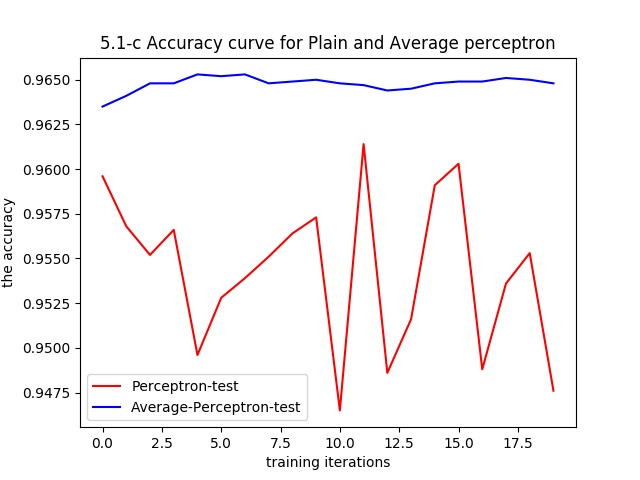
\includegraphics[height=10cm] {part1_c}
			\par	  I find the accuracy of average perceptron is much more stable than the plain perceptron. The plain perceptron and Passive-Aggressive algorithm both appear a shock on the accuracy curve but the average perceptron doesn't.
			\par d.	\par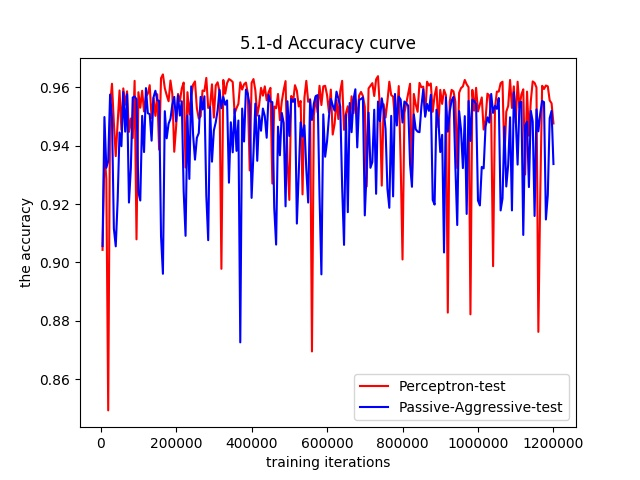
\includegraphics[height=10cm] {part1_d}
			\par		I find that the Perceptron would have a higher accuracy in such training way and it is also more stable. The Passive-Aggressive is really unstable that it would have a 15\% difference between it's accuracy. But in general, these two algorithm both cannot have a stable accuracy curve, 
		\subsection {Multi-Class Classification}
			\par a.	\par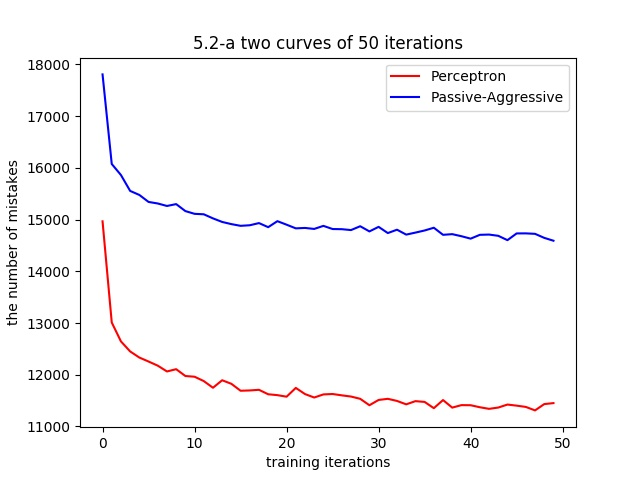
\includegraphics[height=10cm] {part2_a}
			\par I find the number of mistake is much higher than the binary classification. The Passive-Aggressive still have more mistakes than Perceptron. 
			\par b.	\par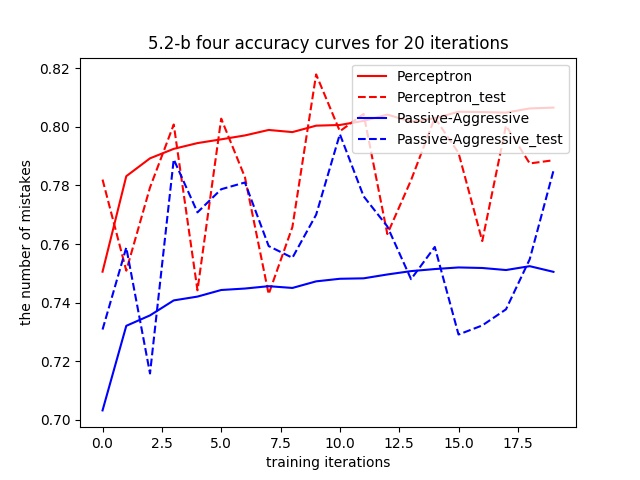
\includegraphics[height=10cm] {part2_b}
			\par With comparing these four curve, I find the Perceptron has higher accuracy than Passive-Aggressive. The curve of training is more stable than test.
			\par c.	\par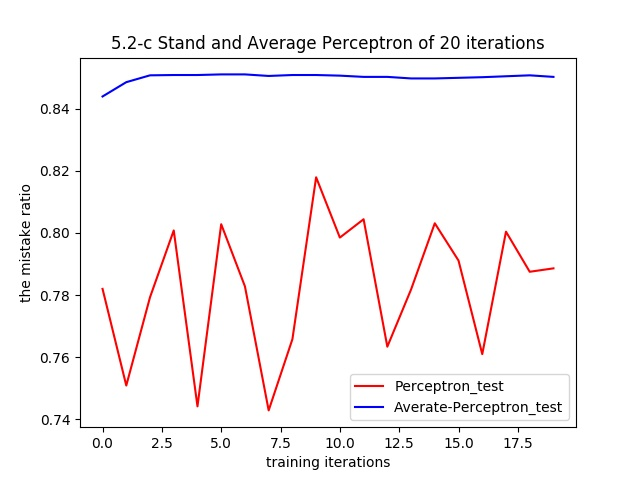
\includegraphics[height=10cm] {part2_c}
			\par The accuracy curve of average perceptron is stable and close to 85\%. Then accuracy curve of Plain Perceptron is not stable and shock between 78\%.
            \par d. 
            \par The result shows that the Average-Perceptron has got a really stable accuracy curve and a high accuracy(85\%), I think it is because every iteration I have done an update to the weight $w$ and reduce the update after test. But the plain perceptron and Passive-Aggressive algorithm are still have a heavy shock around the 80\% and 75\%.
	\section{Summary}
		\par\qquad In the article entitled "A Few Useful Things to Know About Machine Learning", Pedro Domingos reports that Machine Learning is becoming more and more useful and popular nowadays, but it still have a lot of deficiencies and defects. He introduces some basic knowledge and  some matters need attention. Finally, he shows the misunderstandings people may have and some strategy of solving problem.
		\par First of all, the author says that learning is a combination of representation, evaluation and optimization. Representation means people need to make the classifier be a standard format that computers can know. Evaluation function is what people use to confirm whether the classifier is good or not and what they will update. Finally, the optimization is the key to complete the learning process, that is why people separate data to training and test two parts.
        \par But there are still some shortages about the machine learning stratege, it has four mainly challenges. Firstly, it's not enough with data only. Since the machine cannot handle too many classes, which is normal in our real world. So we also need to manage and present the data instead of only asking for large amout of data. Secondly, sometimes we would training too much times and overfitting the data, which is caused by a bad optimization. Then, the dimension is also a question that higher dimension would have a higer accuracy but cost much more time. The last problem is sometimes the real situation is not like in theories. Furthermore, the author also gives some strategy. The first one is catch a efficient feature. The second one is to get more data, which would sometimes lead a better algorithm. The last one is build more models and find the best one to use.
        \par At the end, the author shows some misunderstanding that people may have at the beginning. People usually think complex model would have better performance, but sometimes it's not true. Secondly, sometimes we can get some data from the representable thinks but finally we will find we cannot build model on it. The last misunderstanding is that we may find some data have good correlations but they don't have causations between them, on the contrary, people always think correlation means causation.
        \par In conclusion, this article introduces some basice knowledge and some important things that beginners should pay attention. Beginners of machine learning could know more about machine learning and learn faster with reading this article.
\end{document}
